\documentclass[11pt]{article}
\usepackage{graphicx}
\usepackage{geometry}
\geometry{a4paper, margin=1in}
\usepackage{hyperref}
\usepackage{setspace}
\usepackage{fontspec}
\setmainfont{Cambria}
\usepackage{caption}
\captionsetup[figure]{labelformat=empty, labelsep=none}
\captionsetup[table]{labelformat=empty, labelsep=none}

\begin{document}
\singlespacing
\raggedbottom
\setlength{\parskip}{1em}
\setlength{\parindent}{0pt}

% Cover Page
\begin{titlepage}
    \centering
    \vspace*{1in}
    \Huge
    \textbf{SPIDAM Group Project Report}
    
    \vspace{0.5in}
    \Large
    Group 2
    
    \vfill
    \Large
    \textbf{Date:} \today
    
    \vspace{0.5in}
    \includegraphics[width=0.4\textwidth]{logo.png}
\end{titlepage}

\newpage

% Table of Contents
\tableofcontents
\newpage

% 1. Introduction
\section{Introduction}

% 2.1 Business Needs
\subsection{Business Needs}

The proposed project aims to develop an interactive data acoustic 
modeling tool to assist in the analysis and processing of audio files. 
The primary goal is to create a user-friendly application that allows users to upload, 
clean, and analyze audio files, providing visualizations and metrics such as waveform 
plots and RT60 values. The project is expected to be completed within a three week timeframe, 
requiring basic technical skills in Python programming, audio processing libraries, 
and web development frameworks. The scope includes designing and implementing functionalities 
for file upload, format conversion, data cleaning, and acoustic analysis.

% 2.2 Design Objectives
\subsection{Design Objectives}

The engineering requirements for the project, as stated by the professor or interpreted 
through business needs statements, include the following: the ability to import data by 
loading data files from various sources; providing data cleaning tools to handle missing 
values, remove metadata, and correct inconsistencies in channel format, including 
mp3 to wav format conversion; performing data analysis by generating summary statistics 
and descriptive measures such as the length of audio samples and RT60 values, 
creating data visualizations like histograms, scatter plots, boxplots, or bar charts, 
and visualizing the original waveform; identifying patterns or trends in the data, 
specifically RT60 values over three frequency ranges; data modeling by visualizing model 
performance and interpreting results, visualizing RT60 data for each frequency range and overlapping, 
and displaying the greatest resonant frequency; and reporting by identifying the difference in 
RT60 time to reduce RT60 to a maximum voice intelligibility of 0.5 seconds. The student group will 
also present a report of their project and discoveries.

% 2.3 Functional Requirements
\subsection{Functional Requirements}

The functional requirements for the project are as follows:

\begin{itemize}
    \item The GUI will have a load button to load a sample file.
    \item The system will check for WAV and one other format (MP3 or AAC). If the file is not in WAV format, it will be converted to WAV.
    \item The system will check for metadata (tags) and remove them if present.
    \item The system will check for multi-channel audio. It will handle multi-channel audio or convert it to one channel.
    \item The system will generate six plots: waveform, RT60 for low, mid, and high frequencies, and an additional plot of the user's choice.
    \item The system will provide text output of the time in seconds, the frequency of greatest amplitude, and RT60 differences in seconds.
\end{itemize}

% 2.4 Limitations
\subsection{Limitations}

The project has several assumptions and limitations that need to be considered:

\begin{itemize}
    \item \textbf{Assumptions:}
    \begin{itemize}
        \item Users have basic technical skills in Python programming, audio processing libraries, and web development frameworks.
        \item The audio files provided by users are of sufficient quality and length to perform meaningful analysis.
        \item The system will primarily handle WAV and MP3 file formats, with no support for other audio formats.
        \item The RT60 values calculated will be accurate and representative of the acoustic properties of the audio files.
    \end{itemize}
    
    \item \textbf{Limitations:}
    \begin{itemize}
        \item The project is constrained by a three-week timeframe, which may limit the scope and depth of the functionalities implemented.
        \item The system's performance may vary depending on the hardware and software environment in which it is deployed.
        \item The accuracy of the RT60 values and other metrics may be affected by the quality and characteristics of the input audio files.
        \item The project does not account for real-time audio processing and is intended for offline analysis only.
        \item The system may not handle extremely large audio files efficiently due to memory and processing constraints.
        \item The user interface may be limited in terms of customization and user interaction features.
    \end{itemize}
\end{itemize}

% 3.0 Agile User Stories
\section{Agile User Stories}
\subsection{Epic 1: WAV/MP3 cleaning and processing}

\subsubsection{User Stories}
\begin{itemize}
    \item As a user, I want to upload a WAV file so that I can clean and process it.
    \item As a user, I want it so when I upload a MP3 file, it is converted to WAV form and cleaned.
    \item As a user, I want to clean metadata from a WAV/MP3 file so that I can remove unnecessary information.
\end{itemize}

\subsubsection{Tasks}
\begin{itemize}
    \item Design and implement file upload component
    \item Create and implement MP3 to WAV conversion functionality
    \item Create and implement WAV file cleaning functionality
    \item Create and implement metadata cleaning functionality
\end{itemize}

\subsection{Epic 2: Acoustic Data Analysis}

\subsubsection{User Stories}
\begin{itemize}
    \item As a user, I want to visualize the waveform of an audio file so that I can analyze its characteristics.
    \item As a user, I want to see the RT60 values for low, mid, and high frequencies to understand the reverberation time.
    \item As a user, I want to compare different plots to gain insights into the acoustic properties of the audio.
\end{itemize}

\subsubsection{Tasks}
\begin{itemize}
    \item Create functionality to plot the waveform of an audio file.
    \item Implement backend logic to calculate and plot RT60 values for low, mid, and high frequencies.
    \item Design and implement an additional plot (e.g., bar graph) for comprehensive analysis.
\end{itemize}
% 5. Explanation of each task
\section{Explanation of each task}

\subsection{WAV/MP3 cleaning and processing}

The process of cleaning WAV/MP3 files involves converting MP3 files to WAV 
format using librosa for loading and scipy for saving. Metadata is then removed from the 
WAV files using soundfile to read the audio data and sample rate. This ensures the audio is clear 
and free from unwanted metadata.

\subsection{Acoustic Data Analysis}

The acoustic data analysis involves visualizing the waveform of the audio file using matplotlib
to plot the amplitude of the audio signal over time. RT60 values for low, mid, and high frequencies
are calculated using the Schroeder integration method and plotted to show the reverberation time
across different frequency ranges.

% 6. Results
\section{Results}

\section{Location of Audio Recording}

The audio recording was conducted in the IST. The image below shows the view of the space recorded, including the 
recording position and Aaron Dixon creating the clap.

\begin{figure}[h!]
    \centering
    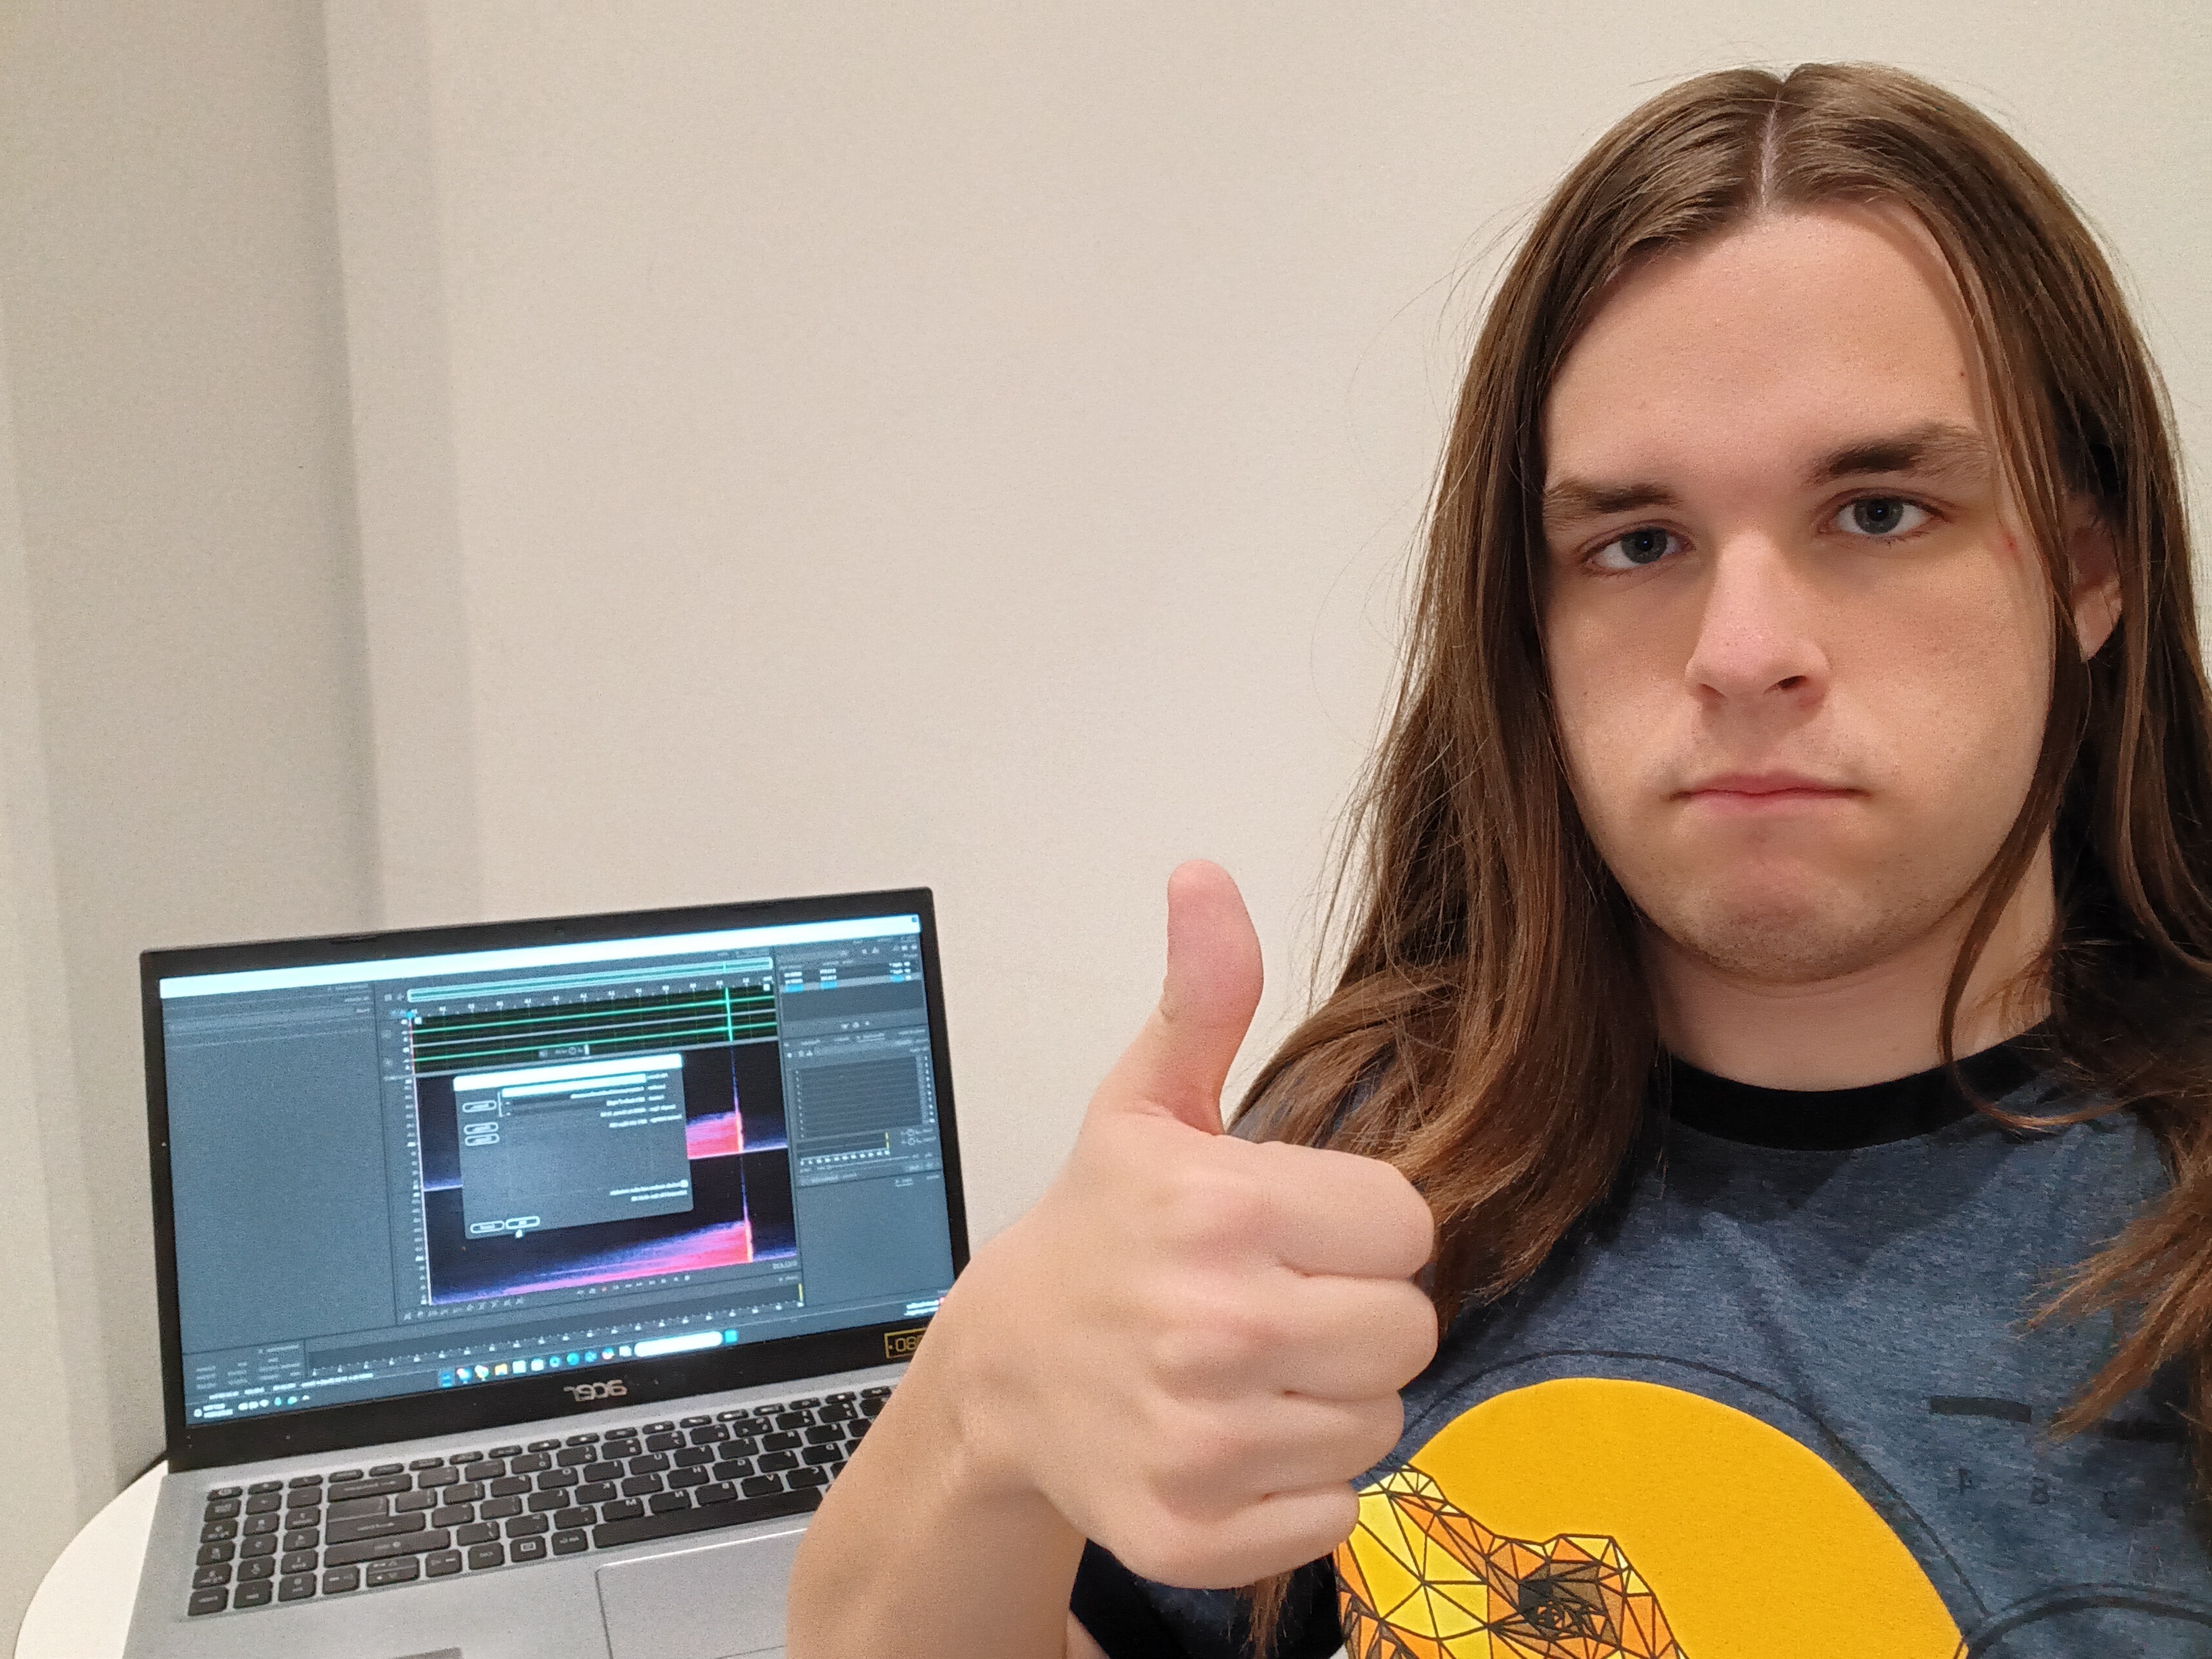
\includegraphics[width=\textwidth]{aaronDixonPic.jpg}
    \caption{Aaron Dixon giving a thumbs up in front of his laptop in the IST building hallway near the 1060 rooms}
\end{figure}

% Numerical Output and Screenshots
\section{Numerical Output and Screenshots}

\subsection{Numerical Output}
The following are the numerical outputs from our measurements:

\begin{itemize}
    \item \textbf{Time in seconds:} 2.63 seconds
    \item \textbf{Frequency of greatest amplitude:} 2134.06 Hz
    \item \textbf{RT60 difference in seconds:} 2.11 seconds
\end{itemize}

\subsection{Screenshots of Plots and Tables}

\begin{figure}[h!]
    \centering
    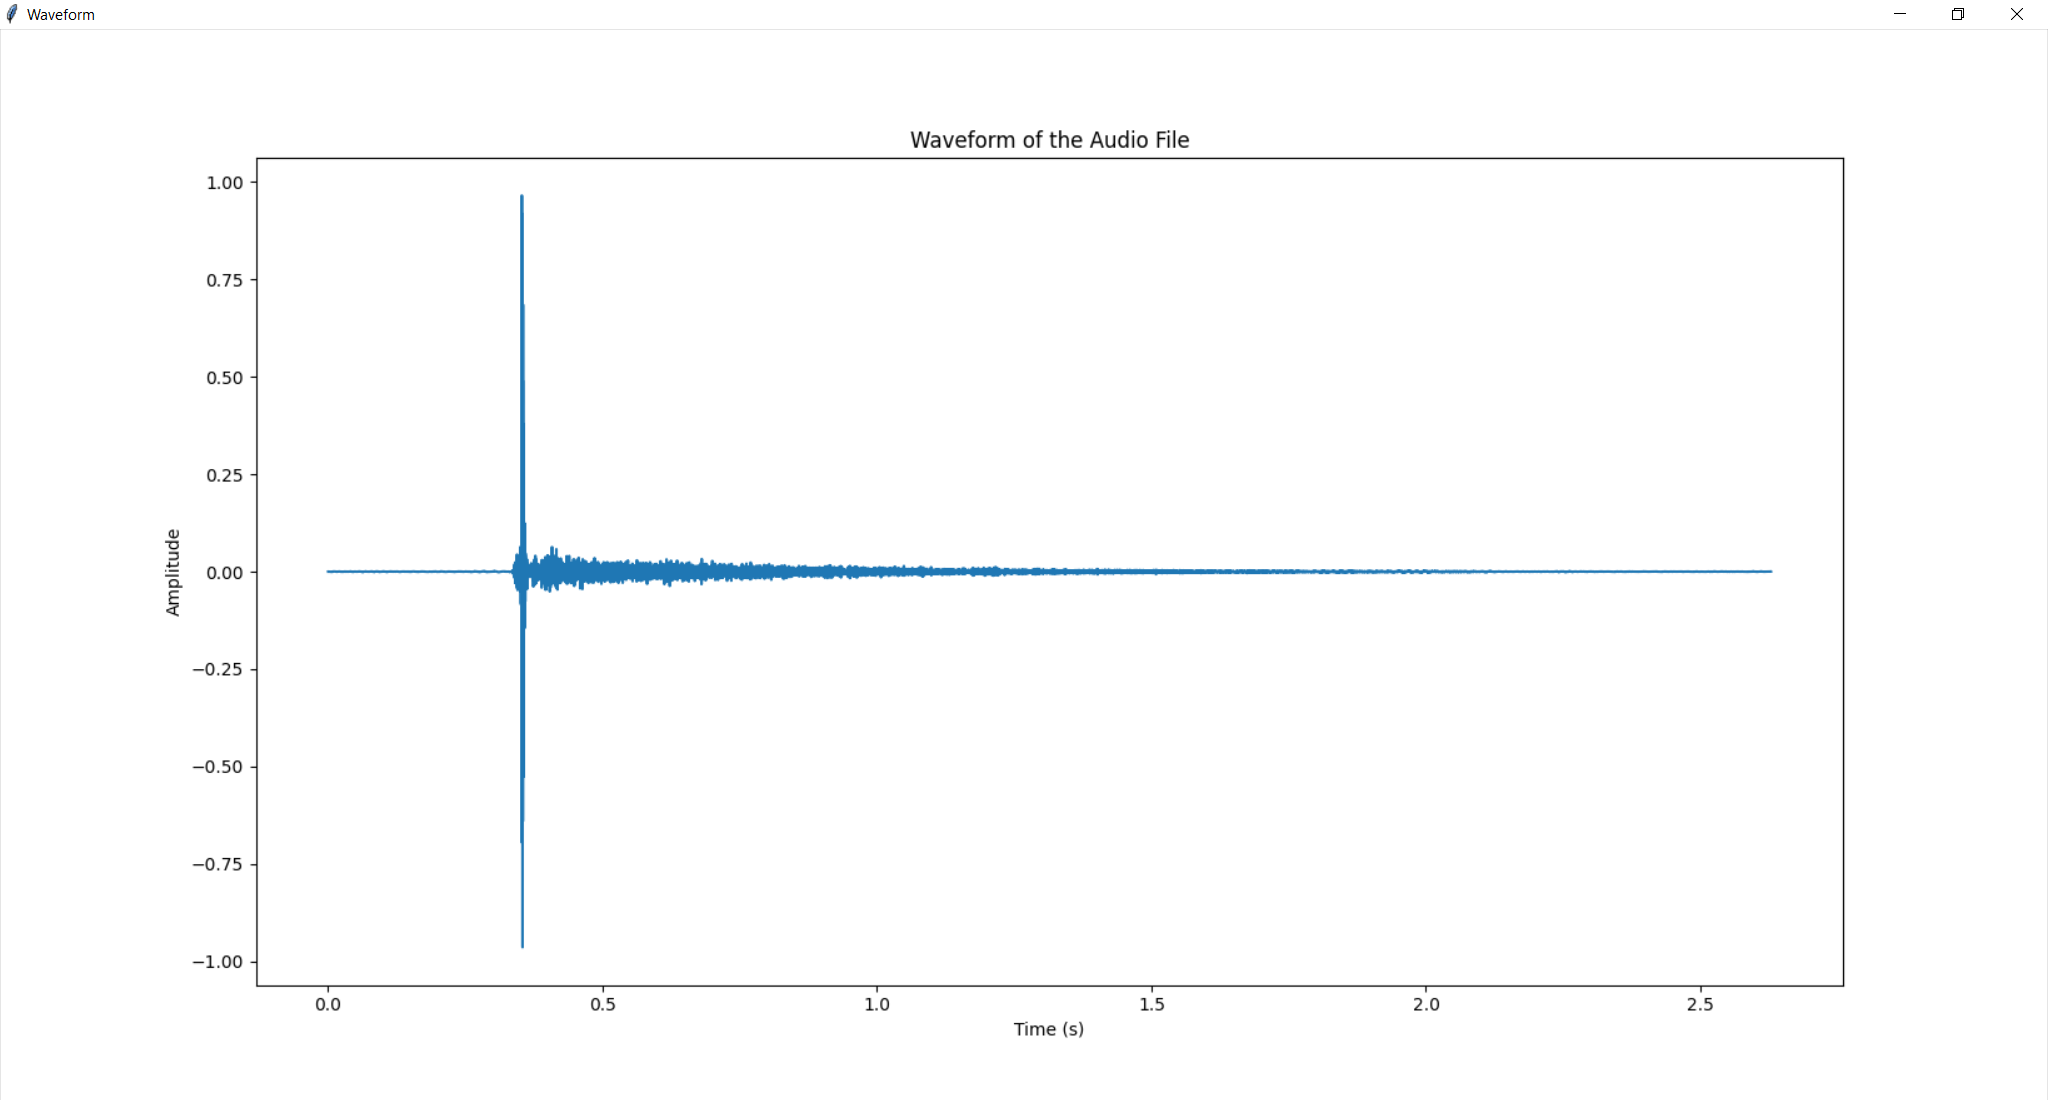
\includegraphics[width=\textwidth]{waveform}
    \caption{Waveform of the audio file}
\end{figure}

\begin{figure}[h!]
    \centering
    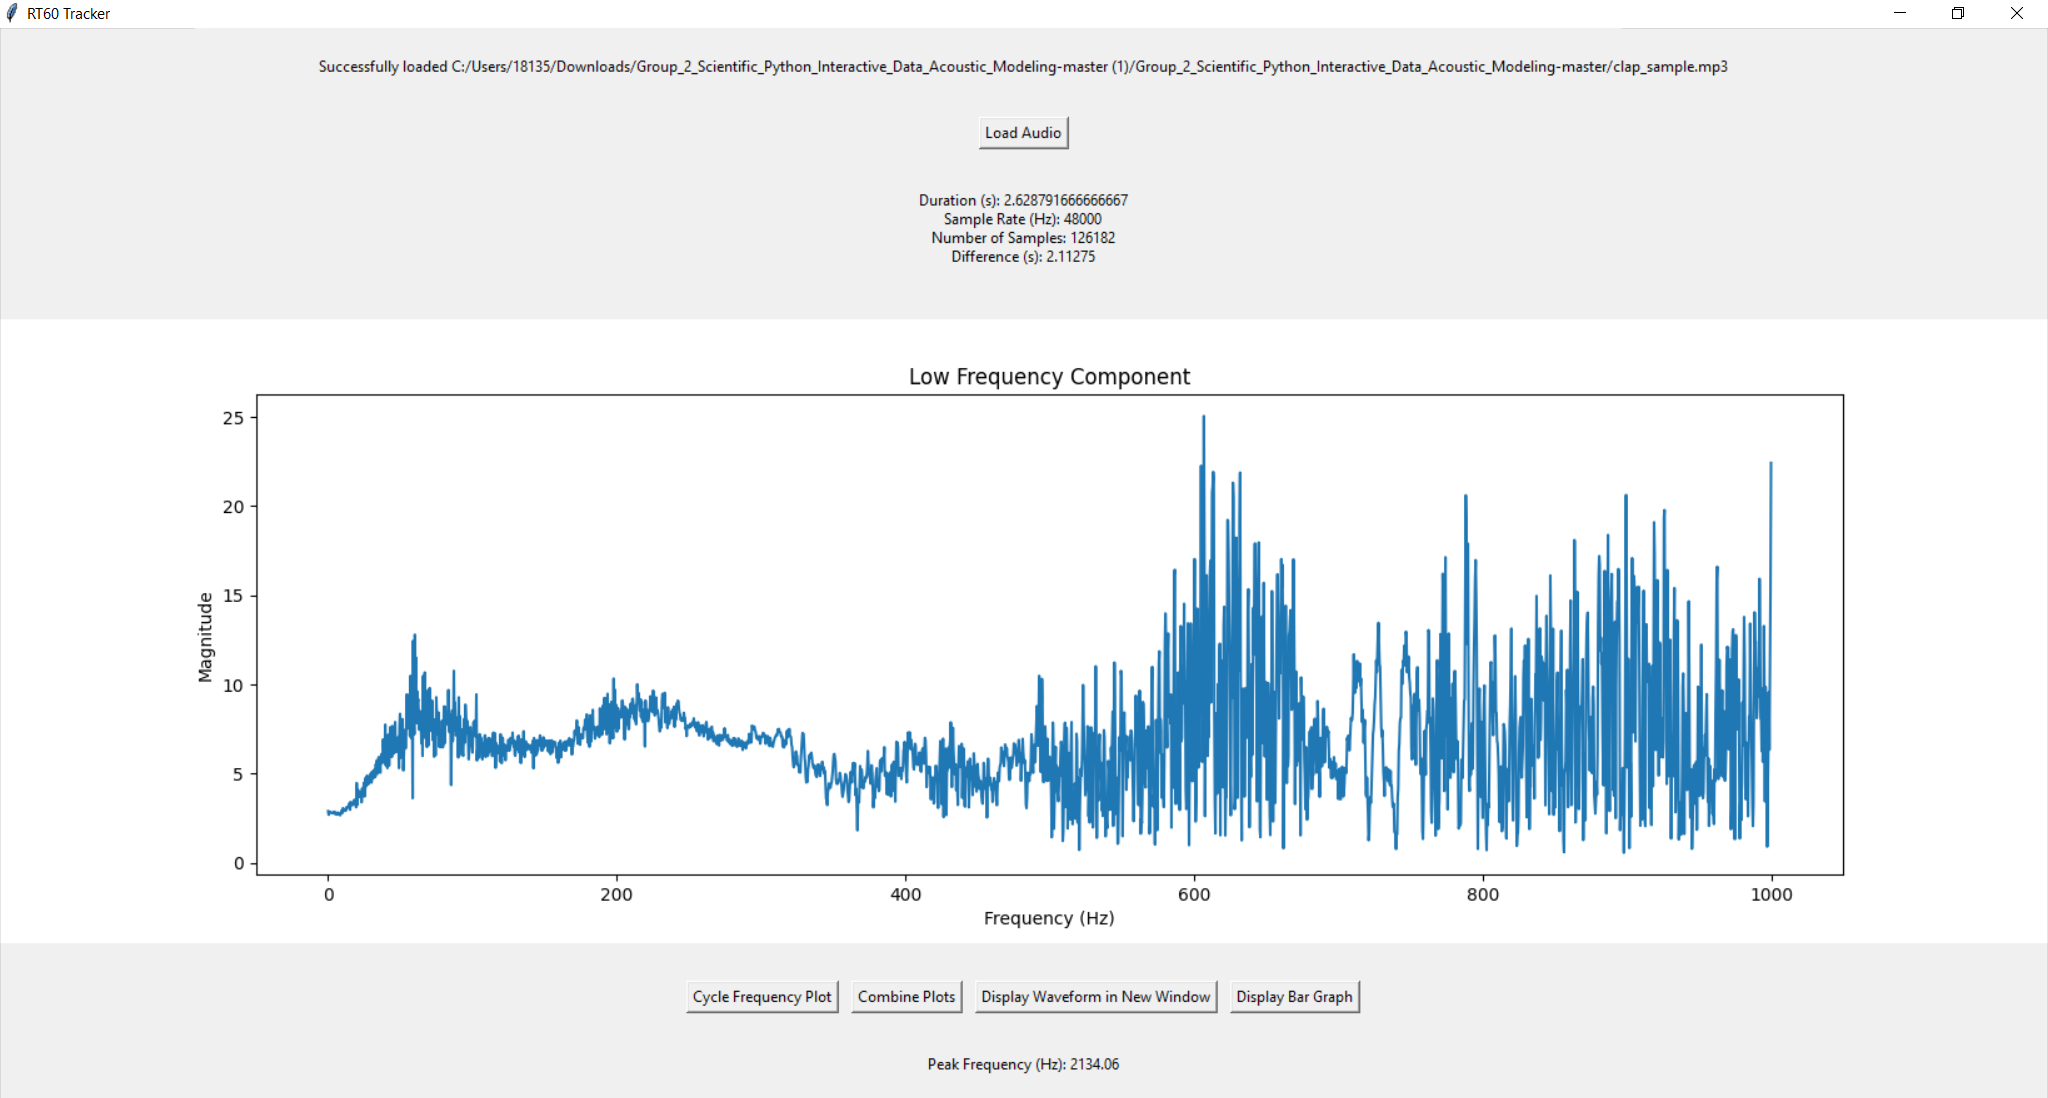
\includegraphics[width=\textwidth]{lowFreq}
    \caption{RT60 for Low Frequency}
\end{figure}

\begin{figure}[h!]
    \centering
    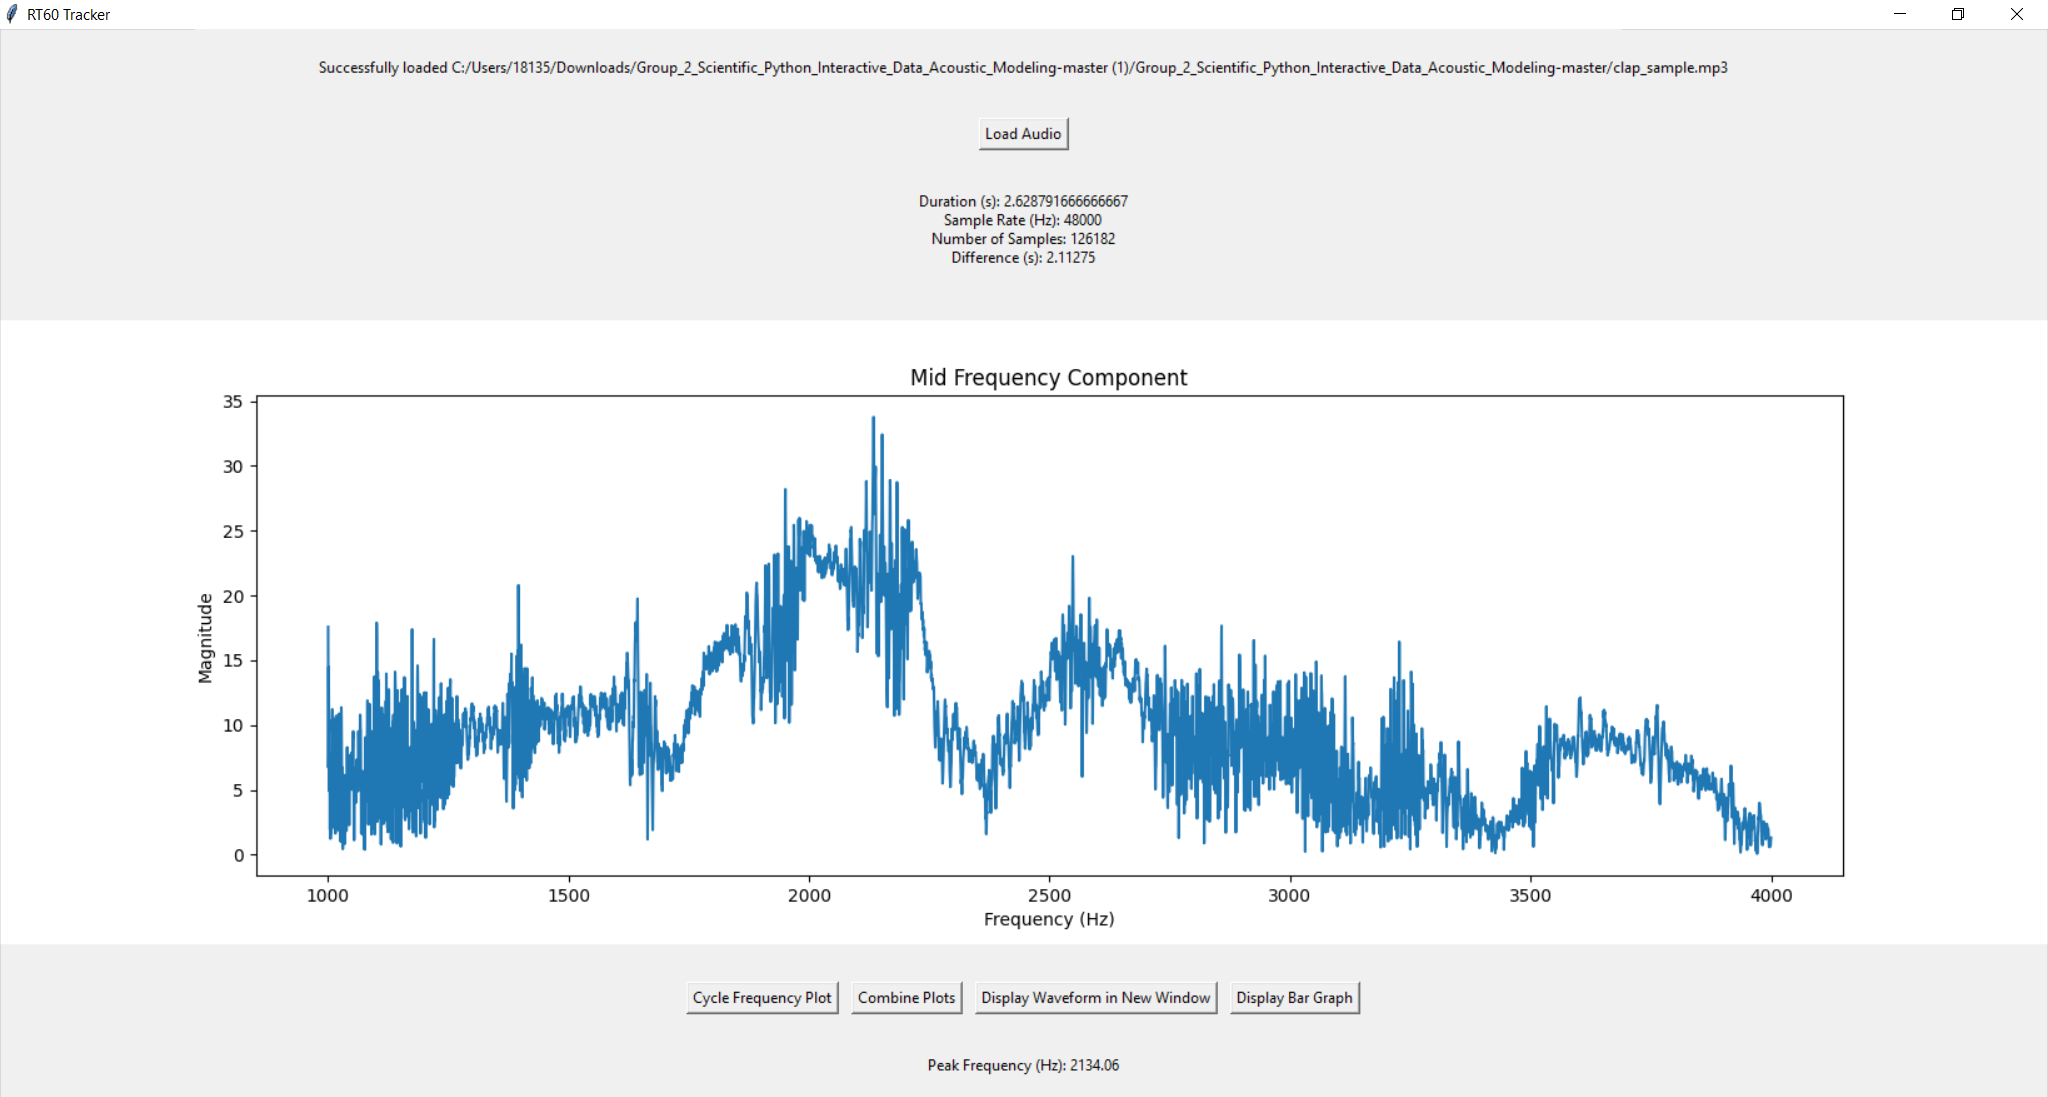
\includegraphics[width=\textwidth]{midFreq}
    \caption{RT60 for Mid Frequency}
\end{figure}

\begin{figure}[h!]
    \centering
    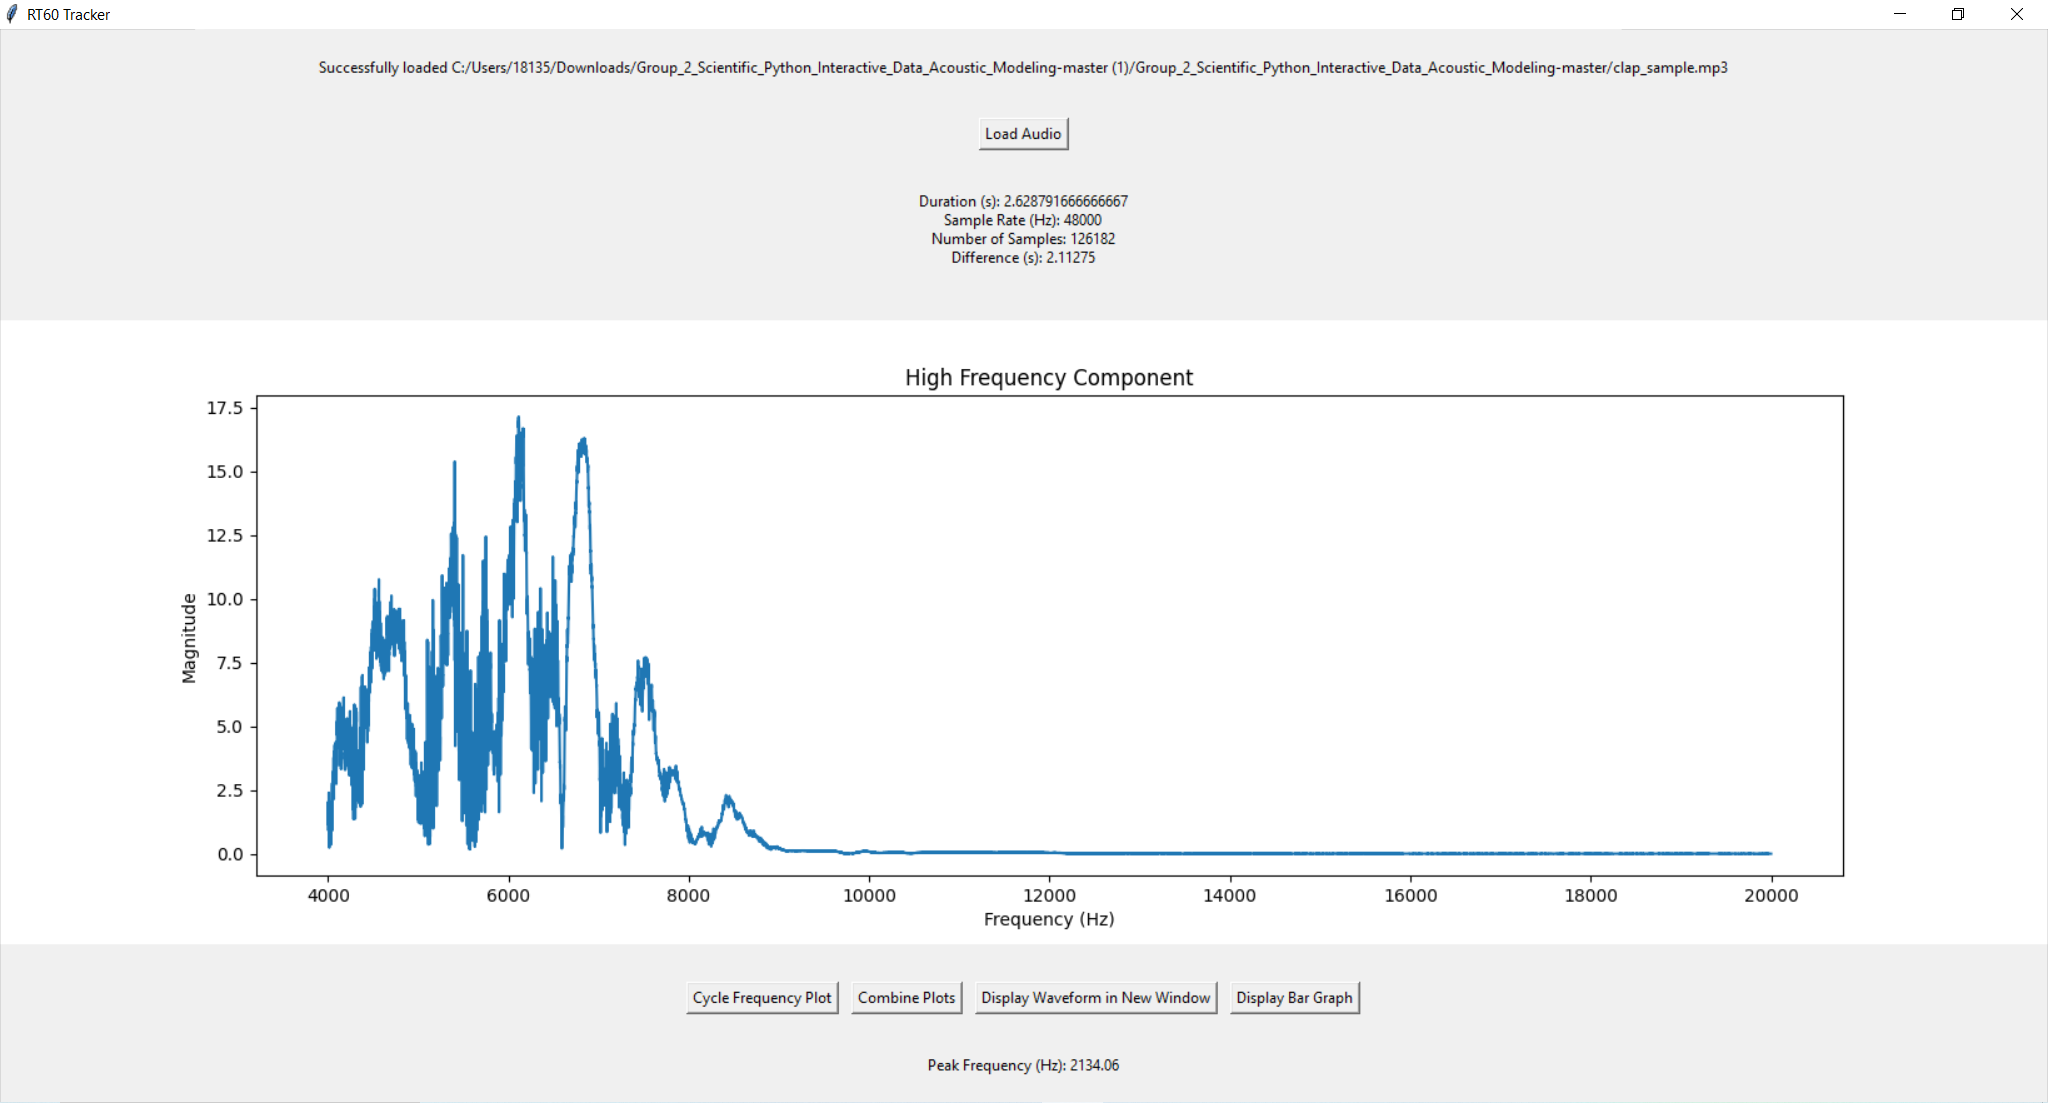
\includegraphics[width=\textwidth]{highFreq}
    \caption{RT60 for High Frequency}
\end{figure}

\begin{figure}[h!]
    \centering
    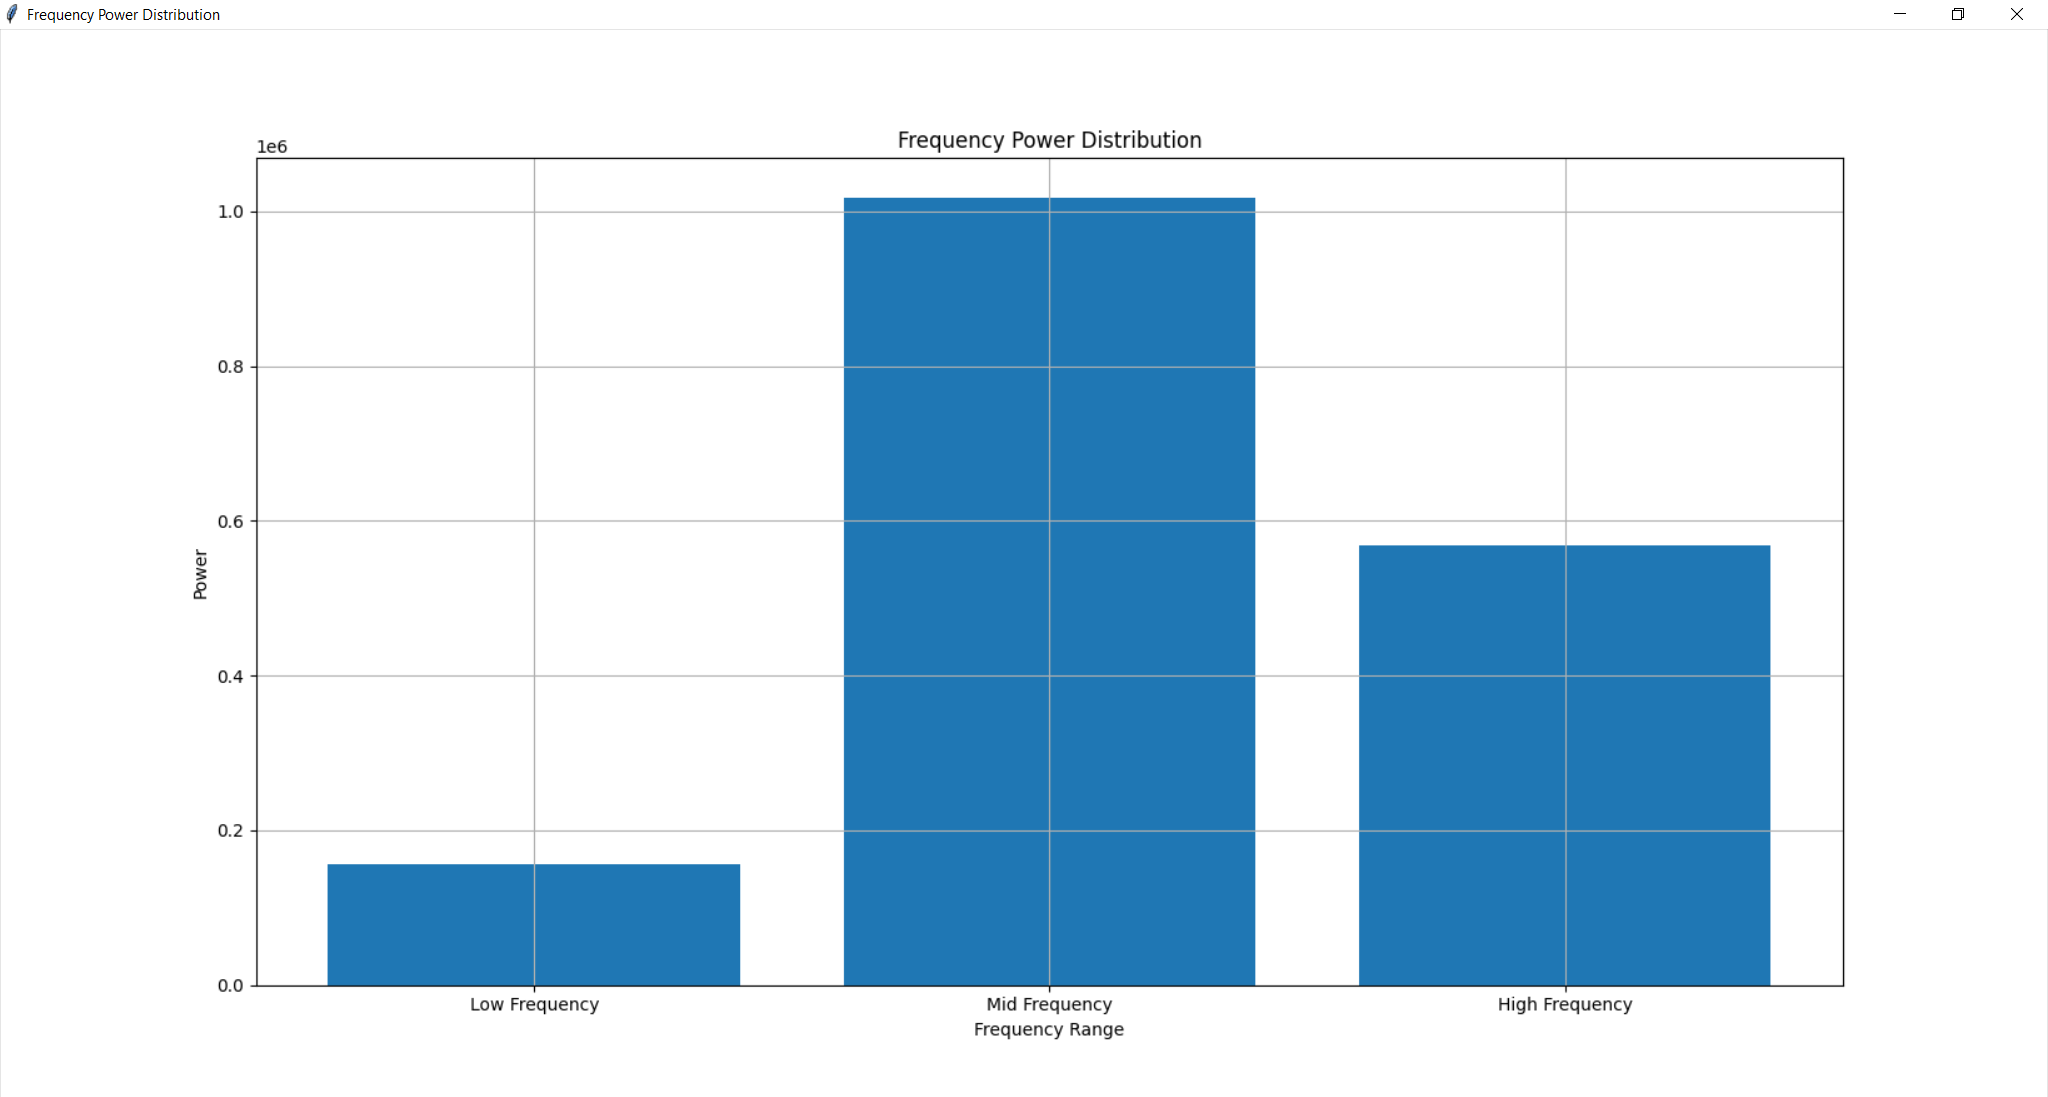
\includegraphics[width=\textwidth]{powerDist}
    \caption{Power Distribution Plot}
\end{figure}

% 6.1 Final Product Testing
\subsection{Final Product Testing}

The final product was tested by running a series of test cases that covered all the functional requirements and design objectives outlined in the project. The testing process involved the following steps:

\begin{itemize}
    \item \textbf{File Upload and Conversion:} We tested the file upload functionality by uploading both WAV and MP3 files. The system successfully converted MP3 files to WAV format and removed metadata as expected.
    \item \textbf{Data Cleaning:} We verified that the system correctly handled multi-channel audio by converting it to a single channel and removed any metadata present in the audio files.
    \item \textbf{Waveform Visualization:} The waveform of the audio files was plotted accurately, showing the amplitude of the audio signal over time.
    \item \textbf{RT60 Calculation and Visualization:} The system correctly calculated and plotted RT60 values for low, mid, and high frequencies, providing insights into the reverberation time of the audio files.
    \item \textbf{Additional Plot:} An additional plot (e.g., bar graph) was generated to provide a comprehensive analysis of the audio data.
    \item \textbf{Text Output:} The system provided text output of the time in seconds, the frequency of greatest amplitude, and RT60 differences in seconds.
\end{itemize}

Overall, the final product met the design objectives and specifications. 
The system was able to handle file uploads, perform necessary conversions and 
cleaning, and generate the required visualizations and metrics. The only 
limitation observed was the performance of the system when handling extremely 
large audio files, which was expected due to memory and processing constraints. 
Despite this, the project successfully achieved its primary goals within the 
given timeframe.

% 7.0 Conclusions and project summary
\section{Conclusions and project summary}

% 7.1 Individual Contribution Table
\subsection{Individual Contribution Table (Based on Git Contributions)}
\begin{table}[h!]
\centering
\caption{Individual Contribution Table}
\begin{tabular}{|c|c|}
\hline
\textbf{Team Member} & \textbf{Contribution Percentage} \\
\hline
Aaron Dixon & 40\% \\
\hline
Rafael Casanova-Silva & 60\% \\
\hline
Kevin Beltran & 0\% \\
\hline
\end{tabular}
\end{table}

% 7.2 Individual contribution reports
\subsection{Individual contribution reports}

\subsubsection{Aaron Dixon}
\subsubsection{Rafael Casanova-Silva}
On November 30th, I forgot about this project to be honest. I was busy with other projects and I didn't have time to work on this one
I made a big push to finish the rest of the code and get the extra credit button done. I also wrote the final report. This would most likely
be not possible without Aaron's help. I'm grateful for his initial contributions in getting the ball rolling and would probably be stumped in
the direction to take without his help. Aaron Dixon has been just awol, and I'm not sure what he's been up to.
\subsubsection{Kevin Beltran}

% 7.3 Individual Reflection reports
\subsection{Individual Reflection reports}

\end{document}